% Chapter Template

\chapter{Descripción del modelo experimental} % Main chapter title

\label{Chapter4} % Change X to a consecutive number; for referencing this chapter elsewhere, use \ref{ChapterX}

\lhead{Capítulo  4. \emph{Descripción del modelo experimental}} % Change X to a consecutive number; this is for the header on each page - perhaps a shortened title

Se definieron 3 modelos experimentales, donde los niveles de abstracción fueron disminuyendo hasta el último, donde se realizaron las pruebas en condiciones reales.\\
El primer modelo, el virtual, representa el sistema en su totalidad en un entorno local, simulando los subsistemas a través de módulos de software.\\
El siguiente fué el modelo físico, donde en cada subsistema se utilizó sobre la arquitectura de \textit{hardware} correspondiente, pero en un entorno de red local.\\
Una vez comprobado que el sistema actuó correctamente en un ambiente físico real aunque limitado, se continuó con el último modelo que fué el real. En este caso, cada sistema se ejecutó en su ambiente real sin limitaciones de conectividad y con la totalidad de sus funcionalidades.\\
En las siguientes secciones se detallan las características de cada modelo.


\newpage


%----------------------------------------------------------------------------------------
%	SECTION 1
%----------------------------------------------------------------------------------------

\section{Modelo virtual}

Como se muestra en la figura \ref{Diagrama_virtual}, este modelo consiste  en probar los subsistemas a través de módulos de \textit{software} ejecutados en la misma computadora, que simulaban el sistema real:\\

\begin{figure}[htbp]
	\centering
		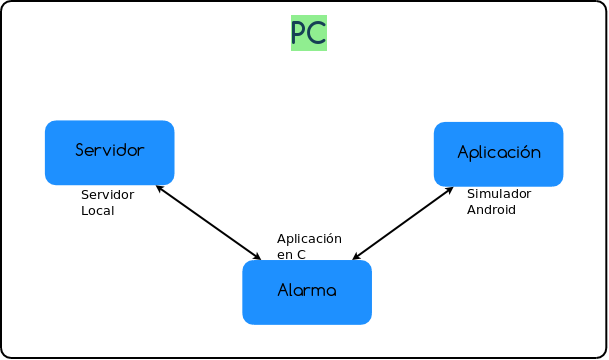
\includegraphics[width=0.8\textwidth]{Figures/Diagrama_virtual.png}
		\rule{35em}{1.5pt}
	\caption[Modelo Virtual del sistema]{Modelo Virtual del sistema}
\label{Diagrama_virtual}
\end{figure}

\begin{figure}[htbp]
	\centering
		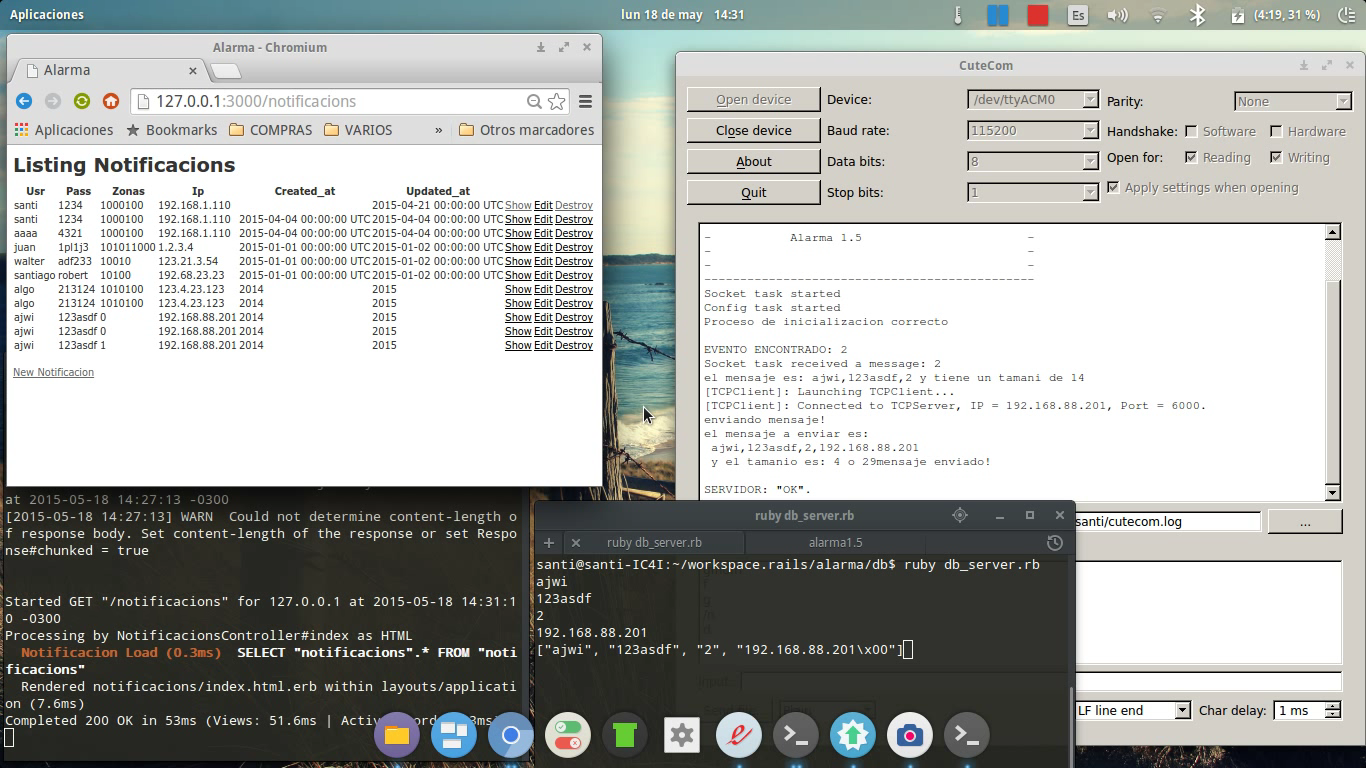
\includegraphics[width=1\textwidth]{Figures/captura_virtual.png}
		\rule{35em}{1.5pt}
	\caption[Captura de pantalla de modelo virtual del sistema]{Captura de pantalla de modelo virtual del sistema}

\end{figure}

A continuación se detalla las funcionalidades básicas propias y de comunicación con el resto de los subsistemas, indicando también, sus limitaciones en cada caso.

\newpage


%-----------------------------------
%	SUBSECTION 1.1
%-----------------------------------
	\subsection{Módulo Alarma}

En el caso de la alarma, se desarrolló un programa en C, que simula las alertas y envía notificaciones al servidor.\\
Limitaciones:
\begin{itemize}
\item Recibe órdenes (activar/desactivar) que simplemente limitan al envío de las notificaciones.
\item No se provee autenticación ni cuenta con salidas para comandar.
\end{itemize}


%-----------------------------------
%	SUBSECTION 1.2
%-----------------------------------

	\subsection{Módulo Servidor}

El servidor, realizado en Ruby sobre el \textit{framework Rails}, integra un \textit{script} que recibe notificaciones por \textit{socket} desde la alarma y las muestra en un servidor \textit{web}.\\
Limitaciones:
\begin{itemize}
\item La interfaz gráfica se limita la exposición de las notificaciones en texto plano.
\item El modelo de la base de datos contempla una única tabla donde se resguardan todos los datos.
\item El controlador del servidor WEB no permite realizar CRUD sobre los datos de los usuarios.
\end{itemize}

%-----------------------------------
%	SUBSECTION 1.3
%-----------------------------------

	\subsection{Módulo Aplicación}

Consta de un \textit{software} hecho en Java sobre el \textit{IDE Android Studio}, que envía ordenes por socket a la alarma y recibe las respuestas de la misma.\\
Limitaciones:
\begin{itemize}
\item Este programa se ejecuta sobre un emulador de teléfonos Android.
\item No permite autenticación.
\end{itemize}

\newpage

%----------------------------------------------------------------------------------------
%	SECTION 2
%----------------------------------------------------------------------------------------

\section{Modelo físico}

Una vez comprobada la funcionalidad en el ambiente virtual, se pasó a un ambiente físico controlado y limitado.
El mismo se representa en la figura \ref{Diagrama_fisico}:

\begin{figure}[htbp]
	\centering
		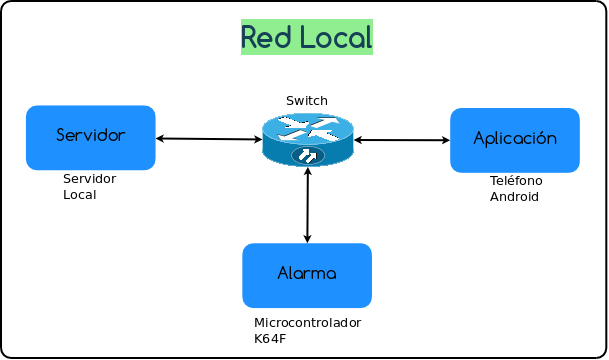
\includegraphics[width=0.8\textwidth]{Figures/Diagrama_fisico.png}
		\rule{35em}{1.5pt}
	\caption[Modelo Físico del sistema]{Modelo Físico del sistema}
\label{Diagrama_fisico}
\end{figure}

Se puede ver que la ejecución del sistema, si bien es sobre la arquitectura correspondiente, la conectividad es limitada a un ambiente de red local y las funcionalidades de cada subsistema no contemplan aún la totalidad de los requerimientos, aunque si los básicos y algunos secundarios.
\newpage


%-----------------------------------
%	SUBSECTION 2.1
%-----------------------------------
	\subsection{Módulo Alarma}

Se desarrolló sobre el microcontrolador K64F, utilizando el \textit{IDE KDS} y el SO \textit{MQX}. \\
Limitaciones:
\begin{itemize}
\item En el caso de los sensores, solo se limitan a interruptores que accionan las alertas, que luego se transmiten en la red local hasta el servidor. 
\item Las notificaciones se restringen a la red local.
\end{itemize}

%-----------------------------------
%	SUBSECTION 2.2
%-----------------------------------

	\subsection{Módulo Servidor}

El servidor se mantuvo en una computadora local, se agregaron funcionalidades \textit{CMS} al servidor \textit{web} para administrar las alarmas y autenticación en las notificaciones entrantes. \\

Limitaciones:
\begin{itemize}
\item Las actualizaciones en la vista del servidor no se realizan automáticamente.
\item Acceso únicamente en red local.
\end{itemize}
\newpage

%-----------------------------------
%	SUBSECTION 2.3
%-----------------------------------

	\subsection{Módulo Aplicación}

Se añadieron múltiples comandos, que se ejecutan directamente desde el teléfono conectado vía \textit{WiFi} a la red local, hacia la alarma. También se mejoró la interfaz de usuario, como se puede ver en la figura \ref{app}:\\

\begin{figure}[htbp]
	\centering
		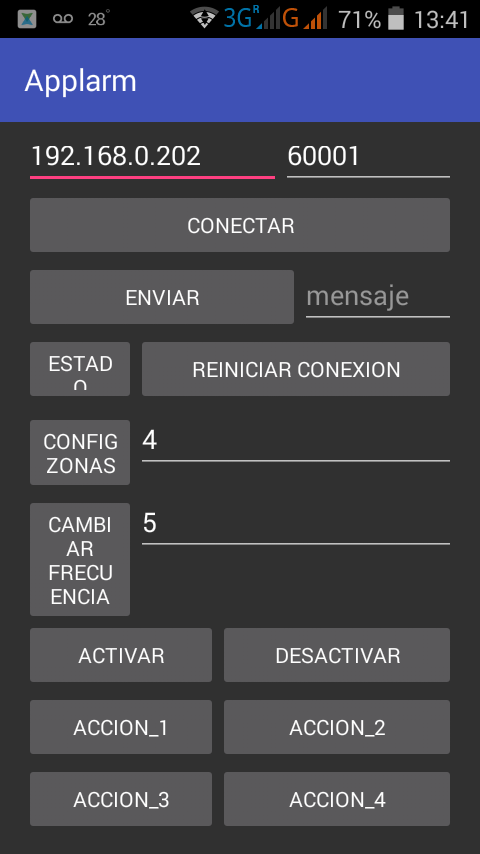
\includegraphics[width=0.5\textwidth]{Figures/app.png}
		\rule{35em}{1.5pt}
	\caption[Captura de App]{Captura de App}
\label{app}
\end{figure}
\newpage

%----------------------------------------------------------------------------------------
%	SECTION 3
%----------------------------------------------------------------------------------------

\section{Modelo real}

En esta etapa, una vez superadas las pruebas en un entorno restringido, se dio comienzo a las pruebas de campo con el prototipo real.\\
Se añadieron algunas mejoras en las interfaces gráficas y nuevas funcionalidades secundarias, detalladas posteriormente.
El esquema se representa a continuación en la figura \ref{Diagrama_real}:\\	

\begin{figure}[htbp]
	\centering
		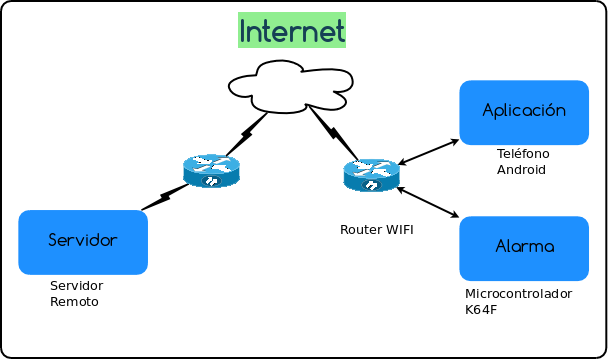
\includegraphics[width=0.8\textwidth]{Figures/Diagrama_real.png}
		\rule{35em}{1.5pt}
	\caption[Modelo Real del sistema]{Modelo Real del sistema}
\label{Diagrama_real}
\end{figure}

\newpage


%-----------------------------------
%	SUBSECTION 3.1
%-----------------------------------
\subsection{Módulo Alarma}

Se agregó la capacidad de comandar elementos externos, a través de un \textit{shield} desarrollado para el microcontrolador.\\
Se añadieron los sensores correspondientes para detectar las alertas.
La figura \ref{pcb} y \ref{relay_shield}, detalla se composición:\\
\begin{figure}[htbp]
	\centering
		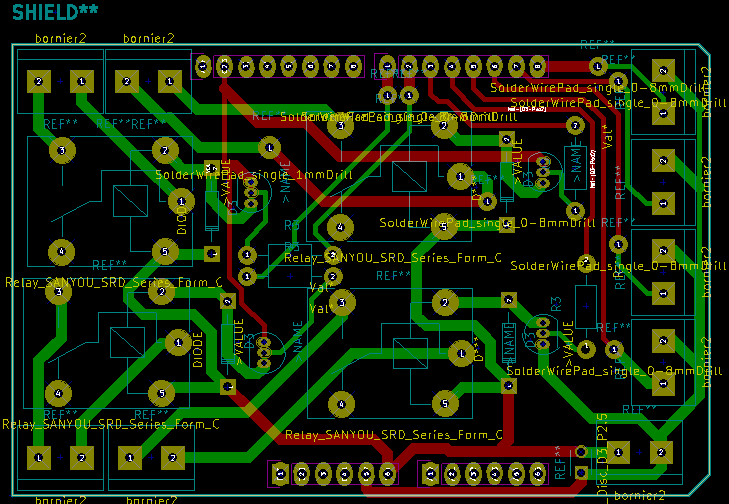
\includegraphics[width=0.8\textwidth]{Figures/pcb.png}
		\rule{35em}{1.5pt}
	\caption[PCB]{PCB}
\label{pcb}
\end{figure}

\begin{figure}[htbp]
	\centering
		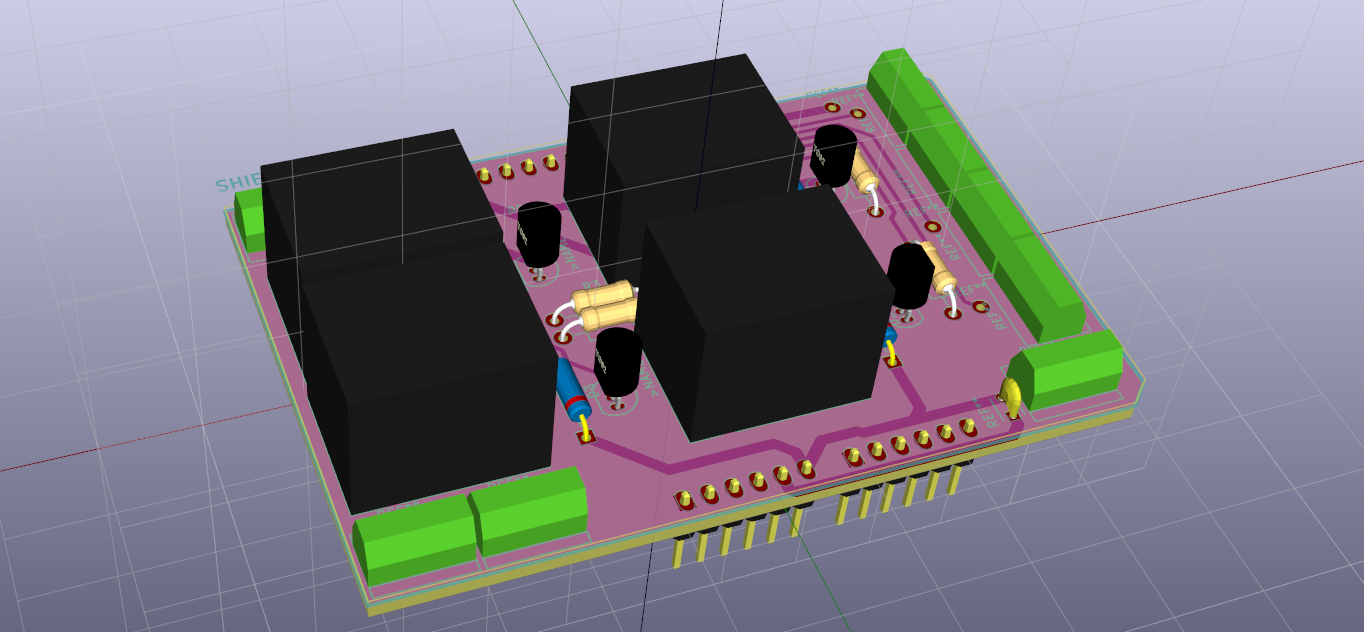
\includegraphics[width=1\textwidth]{Figures/relay_shield.png}
		\rule{35em}{1.5pt}
	\caption[Vista 3D \textit{shield}]{Vista 3D \textit{shield}}
\label{relay_shield}
\end{figure}
\newpage

%-----------------------------------
%	SUBSECTION 3.2
%-----------------------------------

\subsection{Módulo Servidor}

Se montó el servidor, en una \textit{PC} dedicada para tal fin. Para dotarla de acceso remoto se \textit{forwardearon} los puertos del \textit{router} necesarios para que redirigiera las conexiones hacia el servidor.\\
Por otro lado, se utilizó un servicio de \textit{DDNS}, para mantener un dominio fijo y que el servidor pueda ser encontrado ante un cambio de IP (ya que no se contaba con una dirección IP estática pública).\\
Se añadieron notificaciones automáticas vía \textit{E-mail} a los usuarios de las alarma.\\
Por último, se mejoró el \textit{frontend} como se puede apreciar en la figura \ref{servidor}, con la ayuda de \textit{JavaScript} y se agregó autenticación de usuario para el administrador del sistema. Además se utilizó el \textit{framework Bootstrap} para añadir una mejora gráfica en la interfaz de usuario hecha en HTML5. \\

\begin{figure}[htbp]
	\centering
		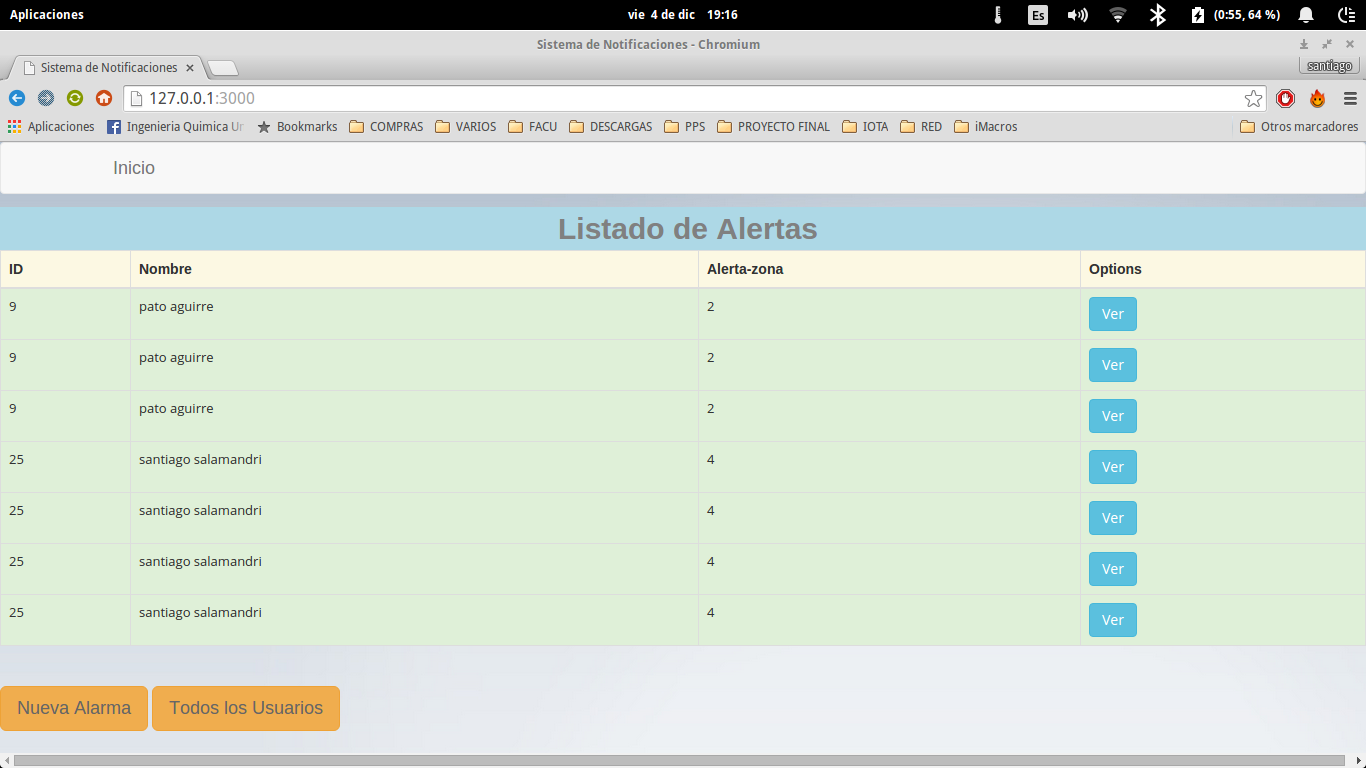
\includegraphics[width=1\textwidth]{Figures/servidor.png}
		\rule{35em}{1.5pt}
	\caption[Servidor]{Servidor}
\label{servidor}
\end{figure}
\newpage

%-----------------------------------
%	SUBSECTION 3.2
%-----------------------------------

\subsection{Módulo Aplicación}

Se mejoró la interfaz gráfica, removiendo botones innecesarios y separando las actividades de configuración de las de comando remoto. En la figura \ref{app_final}, se exhiben los cambios realizados:\\

\begin{figure}[htbp]
	\centering
		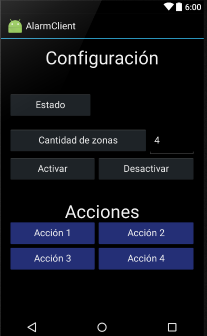
\includegraphics[width=0.5\textwidth]{Figures/app_final.png}
		\rule{35em}{1.5pt}
	\caption[Captura de App final]{App Final}
\label{app_final}
\end{figure}
\newpage